%!TEX root = ../report.tex

\section{Technik}

Generell geht es darum Bewegungsabläufe in Bezug auf Geschwindigkeit und/oder Genauigkeit zu optimieren. Dadurch lassen sich Konditionelle Fähigkeiten optimal ausnutzen, Belastungen reduzieren und das Verletzungsrisiko senken.

\subsection{Begriffe \& Systematik}

Technik ist eine Sammelbezeichnung für eine Reihe technischer Fertigkeiten eines Sportlers/einer Sportart. Eine technische Fertigkeit ist eine erprobte, zweckmäßige und effektive Bewegungsfolge zur Lösung einer definierten Aufgabe in Sportsituationen. Beispiel: Pritschen ist erprobte Bewegungsabfolge der Aufgabe ``Zuspielen'' und teil der technischen Fertigkeiten eines Volleyballers.

Eigenschaften der Technik:
\begin{itemize}
    \item Individualitätseigenschaft: Eindeutige Identifizierung von Weltklasseathleten auf Basis ihrer individuellen Technik
    \item Stabilitätseigenschaft: Technische Fertigkeiten sind hochgeübte Bewegungsfolgen die erst nach Jahren beherrscht werden
    \item Variabilitätseigenschaft: Biomechanische Messungen zeigen immer Variabilitäten, Keine Bewegung entspricht exakt einer anderen und Fähigkeit zur Anpassung der Bewegung während der Ausführung wichtig
\end{itemize}

Es gibt verschiedene Möglichkeiten die Technik zu unterteilen.
Beispiele:
\begin{itemize}
    \item Elementare Fähigkeiten vs. komplexe Sportspezifische Fertigkeiten
    \item Umwelt variabel / konstant vs. mit / ohne Zeitruck
    \item  Sportartspezifische Systematiken (Volleyball: Abwehr, Aufbau, Angriff)
\end{itemize}

Systematiken:
\begin{itemize}
    \item Sporttechnisches Leitbild:
    \begin{itemize}
        \item Idealtechnik: Optimale Bewegungsfolge zur Lösung der Bewegungsaufgabe
        \item Zieltechnik: Für ein Individuum optimale und anzustrebende Bewegungsfolge
    \end{itemize}
    \item Bewegungsnormen:
    \begin{itemize}
        \item Idealnorm: Wissenschaftlich optimale Bewegungsfolge oder Lösungen der Weltbesten
        \item Funktionale Norm: Notwendige Anforderung, um ein Ziel zu erfüllen
        \item Statistische Norm: Wie macht‘s eine vergleichbare Stichprobe?
    \end{itemize}
    \item Technikerwerbstraining: Neulernen bis Automatisierung des dynamischen Optimums
    \item Technikvariationstraining: Varianten und ihr situationsgerechter Einsatz
    \item Technikanpassungstraining: Anpassung an variable Umwelt (Gelände, Raum, Zeit)
    \item Technikabschirmungstraining: Abschirmen gegen  Ermüdung, Gegner und psychischen Druck
\end{itemize}

\subsection{Determinanten}

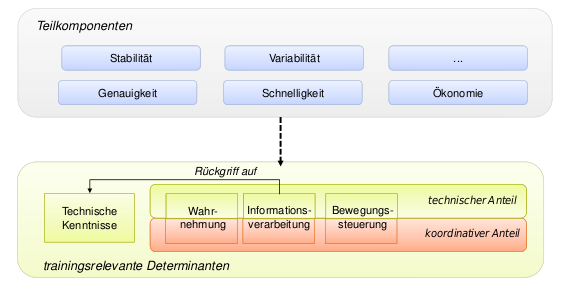
\includegraphics[width=\textwidth]{pictures/tech_determinanten}

\subsubsection*{Phasen des Technikerwerbs}

Das Freiheitsgradproblem:
\begin{itemize}
    \item „Erfunden“ von Nikolai Alexandrowitsch Bernstein, russ. Physiologe, 1896-1966
    \item Problem: Der Mensch hat 880 größere Muskeln!
    \item Wie können diese koordiniert werden?
    \item Motorisches Lernen wird als das Erlernen der Kontrolle von Freiheitsgraden interpretiert: Phasen des motorischen Lernens
\end{itemize}

Phasen des Technikerwerbs:
\begin{enumerate}
    \item Phase ``Freezing'': Einfrieren der Freiheitsgrade
    \begin{itemize}
        \item Freiheitsgrade: Einschränkungen der Muskelgruppen, beteiligter Gelenke, Ausdehnung der Bewegung
        \item Gestalt: geführte Bewegungen, misslingen zunächst öfter
        \item Methodik: Komplexitätsreduktion, Gelegenheit zur Auseinandersetzung geben: Ermüdung, Rückmeldung
    \end{itemize}
    \item Phase ``Releasing'': Befreien der Freiheitsgrade
    \begin{itemize}
        \item Freiheitsgrade:Sukzessives Freisetzen, „selective defrosting“
        \item Gestalt: flüssige, lockere Bewegung, Kombinationen
        \item Methodik: Intensive Rückmeldungen, große Wiederholungszahlen
    \end{itemize}
    \item Phase ``Exploiting'': Ausbeuten der Freiheitsgrade zur Anpassung, Optimierung
    \begin{itemize}
        \item Freiheitsgrade: Ausnutzen, um dynamisches Optimum zu realisieren
        \item Gestalt: oft DVZ, Absprung-, Aushol-, Schlagbewegungen
        \item Methodik: Wann wird zur Ausbeutung gegriffen? Erhöhte Belastung bedenken!
    \end{itemize}
\end{enumerate}

\subsubsection*{Motor Learning}

Lernarten:
\begin{itemize}
    \item Soziales oder Modelllernen: Lernen vom Vorbild, Star, Lehrer, Vormachen-Nachmachen
    \item Versuch-Irrtum-Lernen: Explorierendes Lernen, Implizites Lernen, Bedeutung oft unterschätzt, Anfänger: keine hinreichende Bewegungsvorstellung, Könner: Gegenstand zu differenziert
    \item Lernen durch Einsicht: Zirkel: Instruktion-Durchführung-Ext./Int.Feedback-Bewegungsvorstellung, Umfang und Bedeutung oft überschätzt, Basis des traditionellen methodischen Vorgehens
\end{itemize}

Methodische Übungsreihen (MÜR):
\begin{itemize}
    \item ``Methodische Übungsreihen sind nach methodischen Grundsätzen geordnete Übungsfolgen, die zur Erlernung einer bestimmten motorischen Fertigkeit (Zielübung) ... führen sollen''
    \item Goldstandard des lehrerzentrierten Sportunterrichts
    \item Typen: Aufgliederung in Teilbewegungen, graduelle Annährung, verminderte Lernhilfen
    \item Anordnungsprinzipien: von einfach zu komplex, von leicht zu schwer
\end{itemize}

Neue Ansätze im motorischen Lernen:
\begin{itemize}
    \item bisherige Modelle zu kognitionslastig
    \item Wahrnehmng und Kontext zu wenig berücksichtigt
    \item Bewegungen werden als Antworten auf Umweltkonstellationen interpretiert: ``Constraints'': Einschränkungen der Möglichkeiten, ``Affordances'': Bewegungsmöglichkeiten, diese Wahrnehmung überwiegend unbewusst
    \item Systemdynamischer Ansatz:
    \begin{itemize}
        \item es gibt keine zentrale kortikale Kontrollinstanz zur Bewegungssteuerung
        \item folglich bilden bewusste Prozesse lediglich einen Rahmen für die Bewegungsausführung und sind für die Bewegungskontrolle wenig bedeutsam
        \item Kontrolle wird an dezentrale ``koordinative Strukturen'' delegiert
    \end{itemize}
    \item Ecological approaches: Bewegug wird in einem chaotischen Prozess und in Abhängigkeit von den wechselnden Umweltbedingungen meist unbewusst jedes mal neu generiert. Bewegungslernen = unbewusste Selbstorganisationsprozesse
    \item Implizites Lernen:
    \begin{itemize}
        \item unbewusstes Lernen, ohne Aufmerksamkeit
        \item inzidentell: Unbeabsichtiges Lernen durch Konfrontation mit Lernsituation, Erfolg nicht herbeiführbar (Straßenfußballer-Hypothese)
        \item erfordert intensive und umfangreiche Beschäftigung und hohe Motivation
        \item experimentelle Befunde in der Psychologie
        \item besonders geeignet für komplexe und nicht zu verbalisierende Lerngegenstände
    \end{itemize}
\end{itemize}

Indikationen:
\begin{description}
    \item [Explizit / intentional] bewusstseinspflichtige (erste Lernphasen?) und bewusstseinsfähige Inhalte (Spielzüge, Konzeptionen, Standardsituationen), besonders in kompositorischen und konditionellen Sportarten
    \item [Implizit / inzidentell] komplexe und immer neue Situationen, besonders Sportspiele und Kampfsportarten
\end{description}

\subsection{Trainingsmethoden}

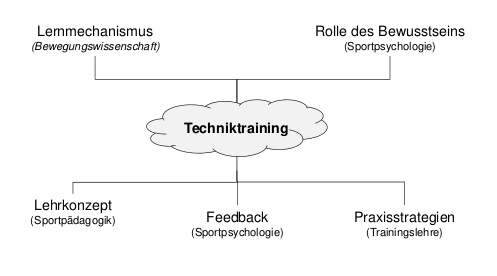
\includegraphics[width=\textwidth]{pictures/tech_mindmap}

\subsubsection*{Lernmechanismus (Bewegungswissenschaft)}

Theorien zum motorischen lernen (die zweite):
\begin{itemize}
    \item Operande Konditionierung (Skinner, 1955): ML ist das Antrainieren von Reflexen auf Umweltreize
    \item Freezing, Releasing, Exploiting (Bernstein,1967): ML ist die Kontrolle von Freiheitsgraden
    \item Motorisch Programme (Schmidt, 1974): ML ist der Aufbau von zentral steuerbaren motorischen Programmen
    \item Theorie der Sensomotorik (Ungerer, 1977): ML ist das Verknüpfen „motorischer Elementarzeichen“ zu Bewegungssequenzen
    \item Ökologische Ansätze (Gibson, 1979, Turvey, 1977): ML ist ein unbewusster Selbstorganisationsvorgang als Antwort auf Umweltwahrnehmungen
\end{itemize}

Lernen durch \ldots:
\begin{itemize}
    \item Konditionierung: Antrainieren von Reflexen (z.B. Deckung beim Boxen), Abtrainieren (Habituation) von Reflexen (z.B. Handballtorwart), Einüben von Bewegungsrhythmen (Stemmschritt)
    \item Imitation: z.B. Fotos, Bildreihen, Videoaufnahmen, Vormachen des Trainers, Beobachtung von anderen Sportlern
    \item Einsicht: Gedankliche Auseinandersetzung mit der eigenen Bewegung, Suchen nach und Erkennen von Fehlern, Erfassen von Ursache und Wirkung, Erarbeitung einer Lösung
    \item Versuch und Irrtum: Lernen muss weitgehend ohne externe Kontrolle/Korrektur funktionieren (z.B. Muttersprache, grundlegende Motorik), Motivation ist nicht das Lernen an sich sondern die Erreichung eines Zieles, Selbständiges Suchen nach Lösungen, Rückschläge in Kauf nehmen, Lernen geschieht hierbei nebenläufig und unbewusst (implizit)
\end{itemize}

\subsubsection*{Lehrkonzept (Sportpädagogik)}

Explizites Techniklernen:
\begin{itemize}
    \item Technik wird wie ein Produkt in mehreren Schritten bewusst (=intentional) ``hergestellt'' (=technologische Position)
    \item Lernen durch Konditionierung, Einsicht, Modellernen, extrinsisches Feedback
    \item Gedankliche Erfassung der Bewegung $\rightarrow$ Beherrschen der Grobform $\rightarrow$ Variation, Stabilisation, Abschirmung
    \item Kritik: ``Kids in America grow up playing in the parks. In Germany they come to the clubs and have practice and stuff like that!''
\end{itemize}

Implizites Techniklernen:
\begin{itemize}
    \item Beiläufiges, ``natürliches'' Lernen ohne Lernabsicht am Einzelfall (=inzidentell)
    \item Antrieb ist eine realen Situation zu lösen
    \item intensive und umfangreiche Beschäftigung, höchst motiviert
    \item Lernen durch Versuch \& Irrtum
    \item ``Freies, unangeleitetes Spielen führt zu Verbesserungen der technischen und taktischen Leistungsvoraussetzungen und ist expliziten Methoden teilweise sogar überlegen'' (Straßenspielerhypothese)
    \item Kritik: Straßenspiel ist zu wenig steuerbar, zu langsam, Erfolg ist unsicher
\end{itemize}

\subsubsection*{Rolle des Bewusstseins (Sportpsychologie)}



\subsubsection*{Feedback (Sportpsychologie)}

\subsubsection*{Praxisstrategien (Trainingslehre)}

\subsection{Trainingsinhalte}

\subsection{Anwendung}

\subsection{Diagnostik}


